As can be seen in Figure \ref{fig:CleavingFiberEnd}, a slightly darkened zone at the bottom of the fiber is observed. This is an unavoidable effect of the cleaving process on plastic fibers, which produces unpolished end-surfaces. To polish the end-surfeces, a method implemented by Thorlabs was applied \cite{DiamondThorlabs}. 

\textbf{Manual Polishing Method.}

The Thorlabs polishing method consists in rubbing the fibers ends with five different polishing papers made of aluminium oxyde grains with a decreasing grain size ($30~\mu\meter$, $20~\mu\meter$, $12~\mu\meter$, $5~\mu\meter$ and $0.3~\mu\meter$). To polish the fiber, this is placed into a polishing connector, shown in Figure \ref{fig:HandPolishingMethod}, and a shape of an 8 must be outlined on each polishing papers during 2 minutes (approximately 120 movements). 

\begin{figure}[h]
\centering
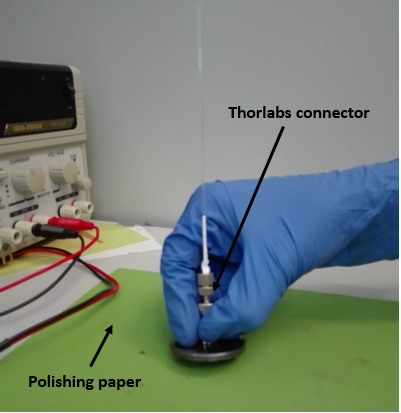
\includegraphics[scale=0.75]{4ResearchAndDevelopments/41Fibers/Hand_Polishing_Kit.png}
\caption{Manual polishing method implemented by Thorlabs.\label{fig:HandPolishingMethod}}
\end{figure}
The result obtained after polishing is shown in Figure \ref{subfig:PolishFiberEnd}, where it can be noticed that the darkened zone has completely disappeared and the fiber end is uniform, which favors optimal coupling and transmision of photons of the scintillating fibers to the photodetectors.

\begin{figure}
\centering
    \begin{subfigure}[b]{0.5\textwidth}
    \centering
    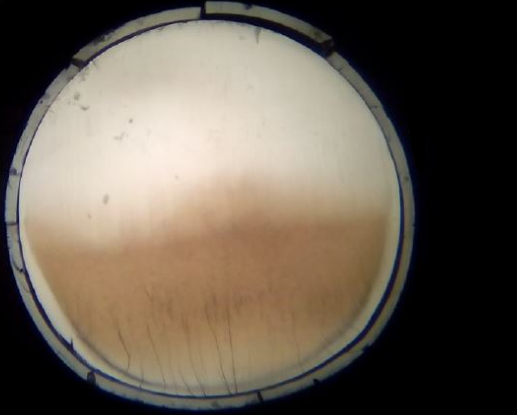
\includegraphics[width=\textwidth]{4ResearchAndDevelopments/41Fibers/CutEndFiberGood.png}  
    \caption{\label{subfig:CleaveFiberEnd}}
    \end{subfigure}
    \hfill
    \begin{subfigure}[b]{0.45\textwidth}
    \centering
    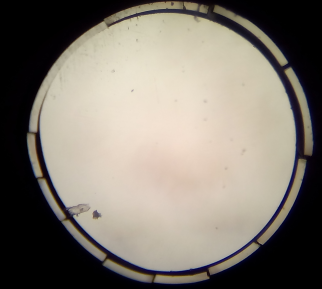
\includegraphics[width=\textwidth]{4ResearchAndDevelopments/41Fibers/CutAndPolishedFiberEnd.png}  
    \caption{\label{subfig:PolishFiberEnd}}
    \end{subfigure}
 \caption{Result of the polishing process. a) Fiber end after cleaving b) Fiber end after cleaving and manual polishing with Thorlabs technique. Pictures taken with the microscope PB 4161 from EUROMEX.}
 \label{fig:ResultofPolishingProcess}
\end{figure}

\textbf{Automatic Polishing Machine.}

The main drawback of the manual polishing method is that it takes more than 10 minutes to polish a fiber. This implies an unaffordable time to polish the thousands of fibers needed for the TRITIUM detector (see section \ref{sec:TritiumMonitor}). For this reason, an automated polishing process was developed within this thesis work. 

%As mentioned above, tens of thousands of fibers had to be prepared and conditioned for the TRITIUM monitor\footnote{Tritium monitor is composed of several modules based on hundred of scintillating fibers.} (see section \ref{sec:TritiumMonitor}). Cleaving this large number of fibers with out home-made cleaving device was a relatively fast process. Polishing them however is quite time consuming, as it takes ten minutes to hand polish one fiber. Hand polishing thoudands of fibers,  would result in an unaffordable amount of time. This is why an automated polishing process has been developed within this thesis work. The goal of this effort was to ensure a better light coupling and transmission of light of the scintillating fibers to the photosensors. 

A machine was designed and built in the laboratory for automatically polishing up to one hundred plastic scintillating fibers at the same time. This machine is easily scalable to larger number of fibers. This automatic polishing machine, displayed in Figure \ref{fig:GeneralViewPolishingMachine}, consists of two main parts:

\begin{figure}[h]
\centering
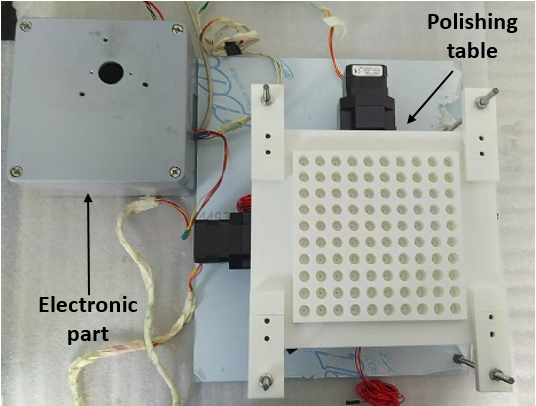
\includegraphics[scale=0.75]{4ResearchAndDevelopments/41Fibers/GeneralViewPolishingMchine.png}
\caption{Polishing machine developed for TRITIUM.\label{fig:GeneralViewPolishingMachine}}
\end{figure}

\begin{enumerate}
\item{} A polishing table, shown in Figure \ref{subfig:PolishingTable}, where the fibers are polished. This is composed of two parts, a static part, to which the fibers are attached, and a movable part on bottom of the previous one, where the polishing papers are fixed. It was decided to move the polishing paper instead of the fibers to avoid damaging them.

The static part that holds the fibers, shown in Figure \ref{subfig:PolishingTable}, consists of a plastic piece locked to the system by four vertical screws. There are two nuts on each screw used to set the relative height and the inclination of fibers relative to the polishing paper. This piece contains one hundred holes in which a hundred fibers are lodged. 

As the fibers are too light ($0.16~\gram$) to make the necessary pressure on the polishing paper by gravity, a plastic belt and a piece of metal of about $1.5~\gram$ weight were attached to the individual fibers, as shown in Figure \ref{subfig:FiberMetailcPiece}, to increase their contact pressure, in a similar way as with manual polishing connectors. 

The movable part of the polishing table consists of a flat PMMA plate of $18 \times 18~\cm^2$ to which the polishing paper is attached. This part is locked to a structure \cite{StructureAxis} that contains two horizontal screws, perpendicular to each other, which allow a movement in the horizontal plane, as shown in Figure \ref{subfig:HorizontalAxis}.

The polishing system contains several high accuracy switches, model DB1 6A250, shown in Figures \ref{subfig:PolishingTable}, \ref{subfig:HorizontalAxis} and \ref{subfig:3DSwitchPiece}, which are used to find the origin of coordinates when the system is reinitiated and to stop the movable part when the end of the path is reached. 

\begin{figure}
\centering
    \begin{subfigure}[b]{0.55\textwidth}
    \centering
    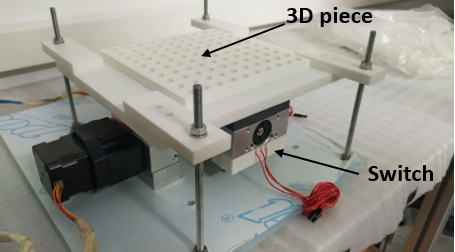
\includegraphics[width=\textwidth]{4ResearchAndDevelopments/41Fibers/PolishingTable.png}  
    \caption{\label{subfig:PolishingTable}}
    \end{subfigure}
    \hfill
    \begin{subfigure}[b]{0.3\textwidth}
    \centering
    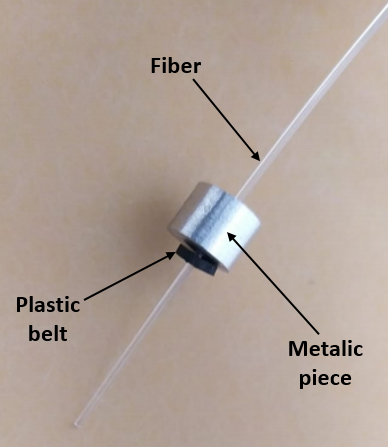
\includegraphics[width=\textwidth]{4ResearchAndDevelopments/41Fibers/PieceOfFiber.png}  
    \caption{\label{subfig:FiberMetailcPiece}}
    \end{subfigure}
    \hfill
    \begin{subfigure}[b]{0.55\textwidth}
    \centering
    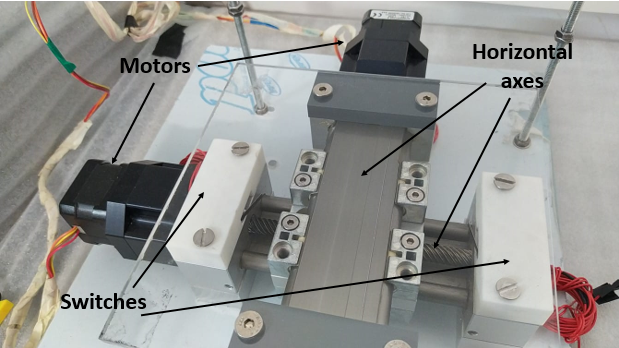
\includegraphics[width=\textwidth]{4ResearchAndDevelopments/41Fibers/HorizontalAxis2.png}  
    \caption{\label{subfig:HorizontalAxis}}
    \end{subfigure}
    \hfill
    \begin{subfigure}[b]{0.4\textwidth}
    \centering
    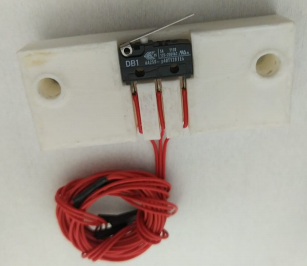
\includegraphics[width=\textwidth]{4ResearchAndDevelopments/41Fibers/Switch.png}  
    \caption{\label{subfig:3DSwitchPiece}}
    \end{subfigure}
 \caption{Components of the fiber polishing machine. a) Polishing table. b) Fiber with ballast metal piece. c) Horizontal screws and PMMA plate. d) A movement switch with its cables inserted inside its holding piece.}
 \label{fig:PolishingTable}
\end{figure}

\item{} An Arduino-based electronics, shown in Figure \ref{fig:ElectronicSystemPolishingMachine}, that controls the movement of the polishing paper. It consists of two stepper motors controlled by an Arduino UNO \cite{ArduinoUNO} that uses a CNC shield \cite{CNCShield}.

%This consists of two stepper motors which move the horizontal screws on which the PMMA plate holding the polishing paper is attached

The stepper motor is a type of DC motor in which a full rotation is divided into a number of steps that define the stepping angle. The stepper motors used for he polishing machine are model NEMA ST4209S1404-A \cite{StepperMotors}, with bipolar voltage of $2.77~\volt_{DC}$, $1.33~\ampere$ maximum current and a stepping angle of $0.9\degree$ ($400$ steps/rev). They can be operated with a position sensor for feedback control. These stepper motors are used to move the horizontal screws on which the PMMA plate that holds the polishing paper is attached.

Two drivers are connected to the CNC shield, which limit the current supplied to the motors. Choosing the right drivers is crucial because overpowering the motors could damage them, while underpowering them would induce an inadequate stepping. Several drivers were succesively tested: the driver Pololu A4988 ($35~\volt$, $2~\ampere$ and $16$ steps) \cite{A4988Driver}, the driver DRV8825 ($45~\volt$, $2.5~\ampere$ and $32$ steps) \cite{DRV8825Driver} and the TMC2208 ($35~\volt$, $2.5~\ampere$ and $256$ steps, with more microstepping modes, which result in a more accurate and smooth movement) \cite{TMC2208Driver}. The last driver includes a StealthChop function that allows the driver to operate in silence mode for low motor velocities. The TMC2208 driver is the one used for the control of the stepper motors since it produce the most accurate and smooth movement. A cooling system, shown in Figure \ref{fig:ElectronicSystemPolishingMachine}, was needed to ensure the correct operation of the polishing system. This consists of a copper heat sink in contact with both controllers and a fan, which prevents heat accumulation inside the electronics box. The cooling power can be improved by a PELTIER cell.

\begin{figure}[h]
\centering
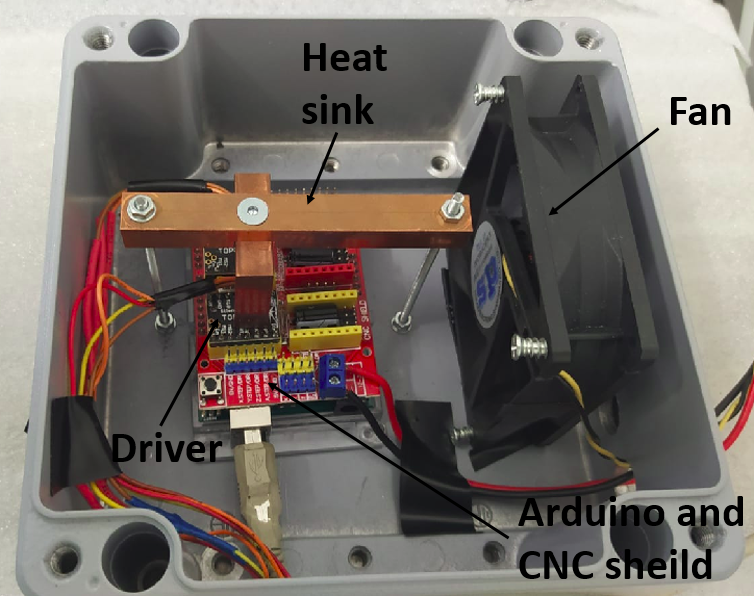
\includegraphics[scale=0.6]{4ResearchAndDevelopments/41Fibers/ElectronicPolishingMachine.png}
\caption{Electronic system of Polishing machine.\label{fig:ElectronicSystemPolishingMachine}}
\end{figure}
\end{enumerate}

The polishing machine is controlled by a Raspberry Pi computer board \cite{RaspberryPi} using the Universal G-code Sender software, a grafical interface based on the GRBL package \cite{GRBLDocumentation}. In this software, there are several pre-programmed functions, such as "HOME" that finds the system origin of coordinates when it is turned on. The GRBL software loads the file containing the G-code that defines the 120 movements required for polishing.

\textbf{Experimental Test.}

The improvement of the light transmission of scintillating fibers due to the polishing process was tested with twenty uncladded scintillating fibers of $15~\cm$ length. These fibers were arranged in a bundle that was coupled to two PMTs and read out in coincidence, as shown in Figure \ref{fig:BunchWith2PMTsCoincidence}.

\begin{figure}[]
\centering
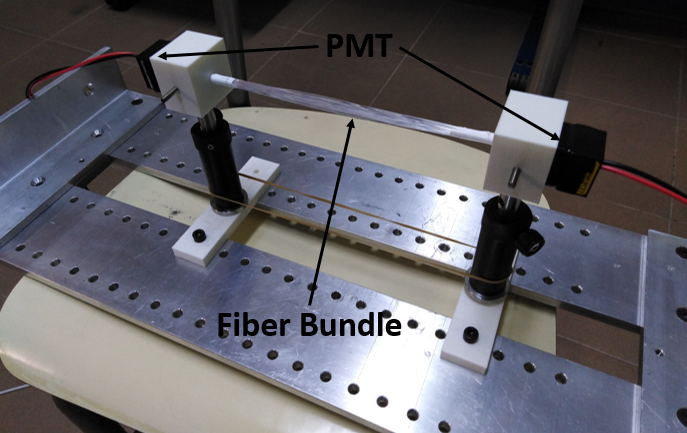
\includegraphics[scale=0.6]{4ResearchAndDevelopments/41Fibers/FiberBunch2PMTsCoincidence.png}
\caption{Setup used to quantify the improvement of the light collection of the fibers and their transmistion to the PMTs due to the polishing process. This setup was placed inside a light-tight box for the measurements.\label{fig:BunchWith2PMTsCoincidence}}
\end{figure}

This experiment was carried out inside a light-tight box, to avoid external light. The spectra produced by background radiation before and after the polishing process are displayed in Figure \ref{fig:ResultsOfPolishingMachineBackground}.
\begin{figure}[]
\centering
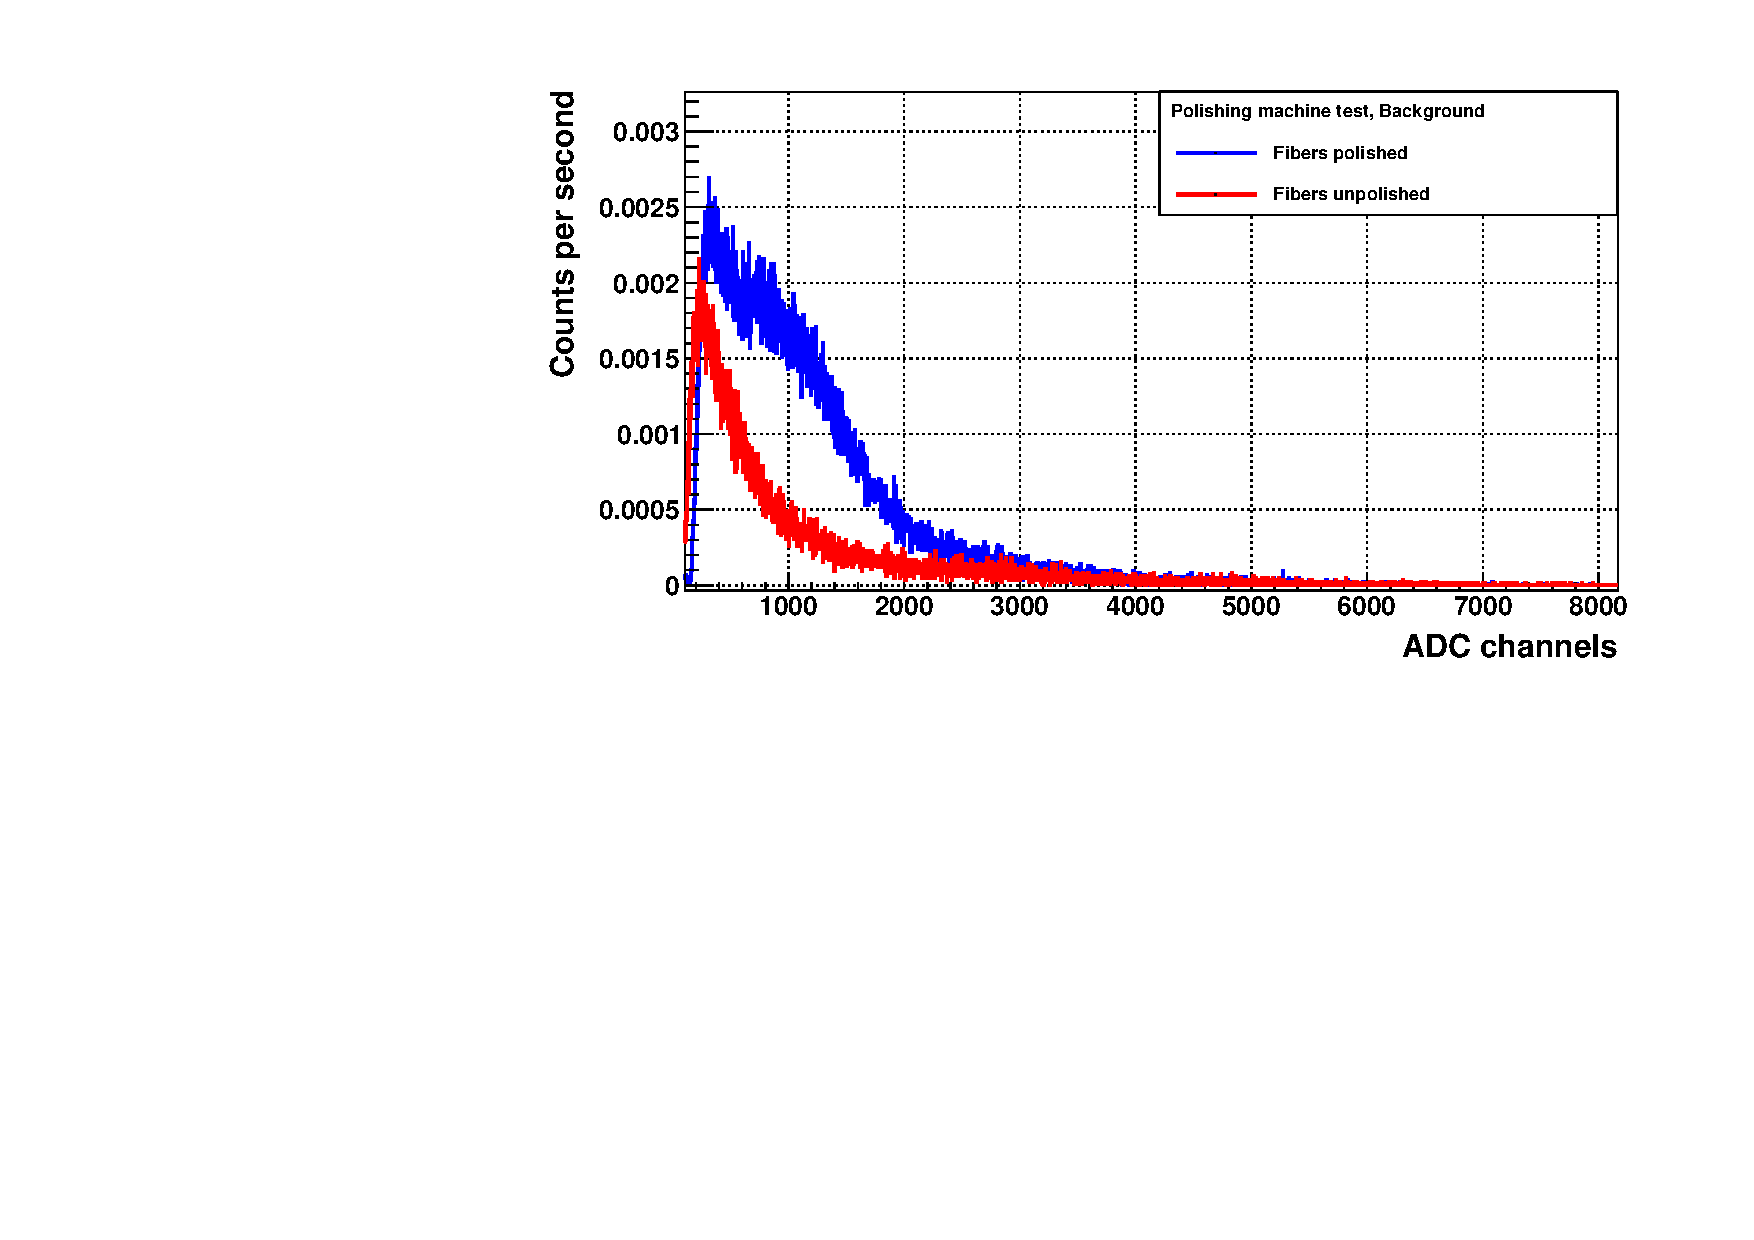
\includegraphics[scale=0.65]{4ResearchAndDevelopments/41Fibers/PolishingTest_Background.pdf}
\caption{Background energy spectra recorded with polished and unpolished fibers.\label{fig:ResultsOfPolishingMachineBackground}}
\end{figure}
As it can be seen in this figure, the energy spectrum after applying the polishing process is shifted to the right, which means that the detected events have more energy than before the polishing process, more photons per event reach the PMTs. The improvement of the photon collection efficiency of the scintillating fibers is quantified by a parameter $F$ defined as,
\begin{equation}
F=\frac{A_{P}}{A_{NP}}
\label{eq:RelativeImprovement}
\end{equation}
where $A_{P}$ and $A_{NP}$ are the integrals of the energy spectrum measured after and before the polishing process, respectively. The polishing results in a factor $2.2$ improvement in light collection. 

The test was repeated with two radioactive sources, an encapsulated $\ce{^{60}Co}$ source of $715~\becquerel$ activity and a $\ce{^{90}Sr}$ source of $17.8~\kilo\becquerel$ activity. The radioactive sources were placed next to the center of the fiber bundle (at $7.5~\cm$ from each PMT). The energy spectra recorded for both radioactive sources are shown in Figure \ref{fig:ResultsOfPolishingMachineSources}.
\begin{figure}
\centering
    \begin{subfigure}[b]{1\textwidth}
    \centering
    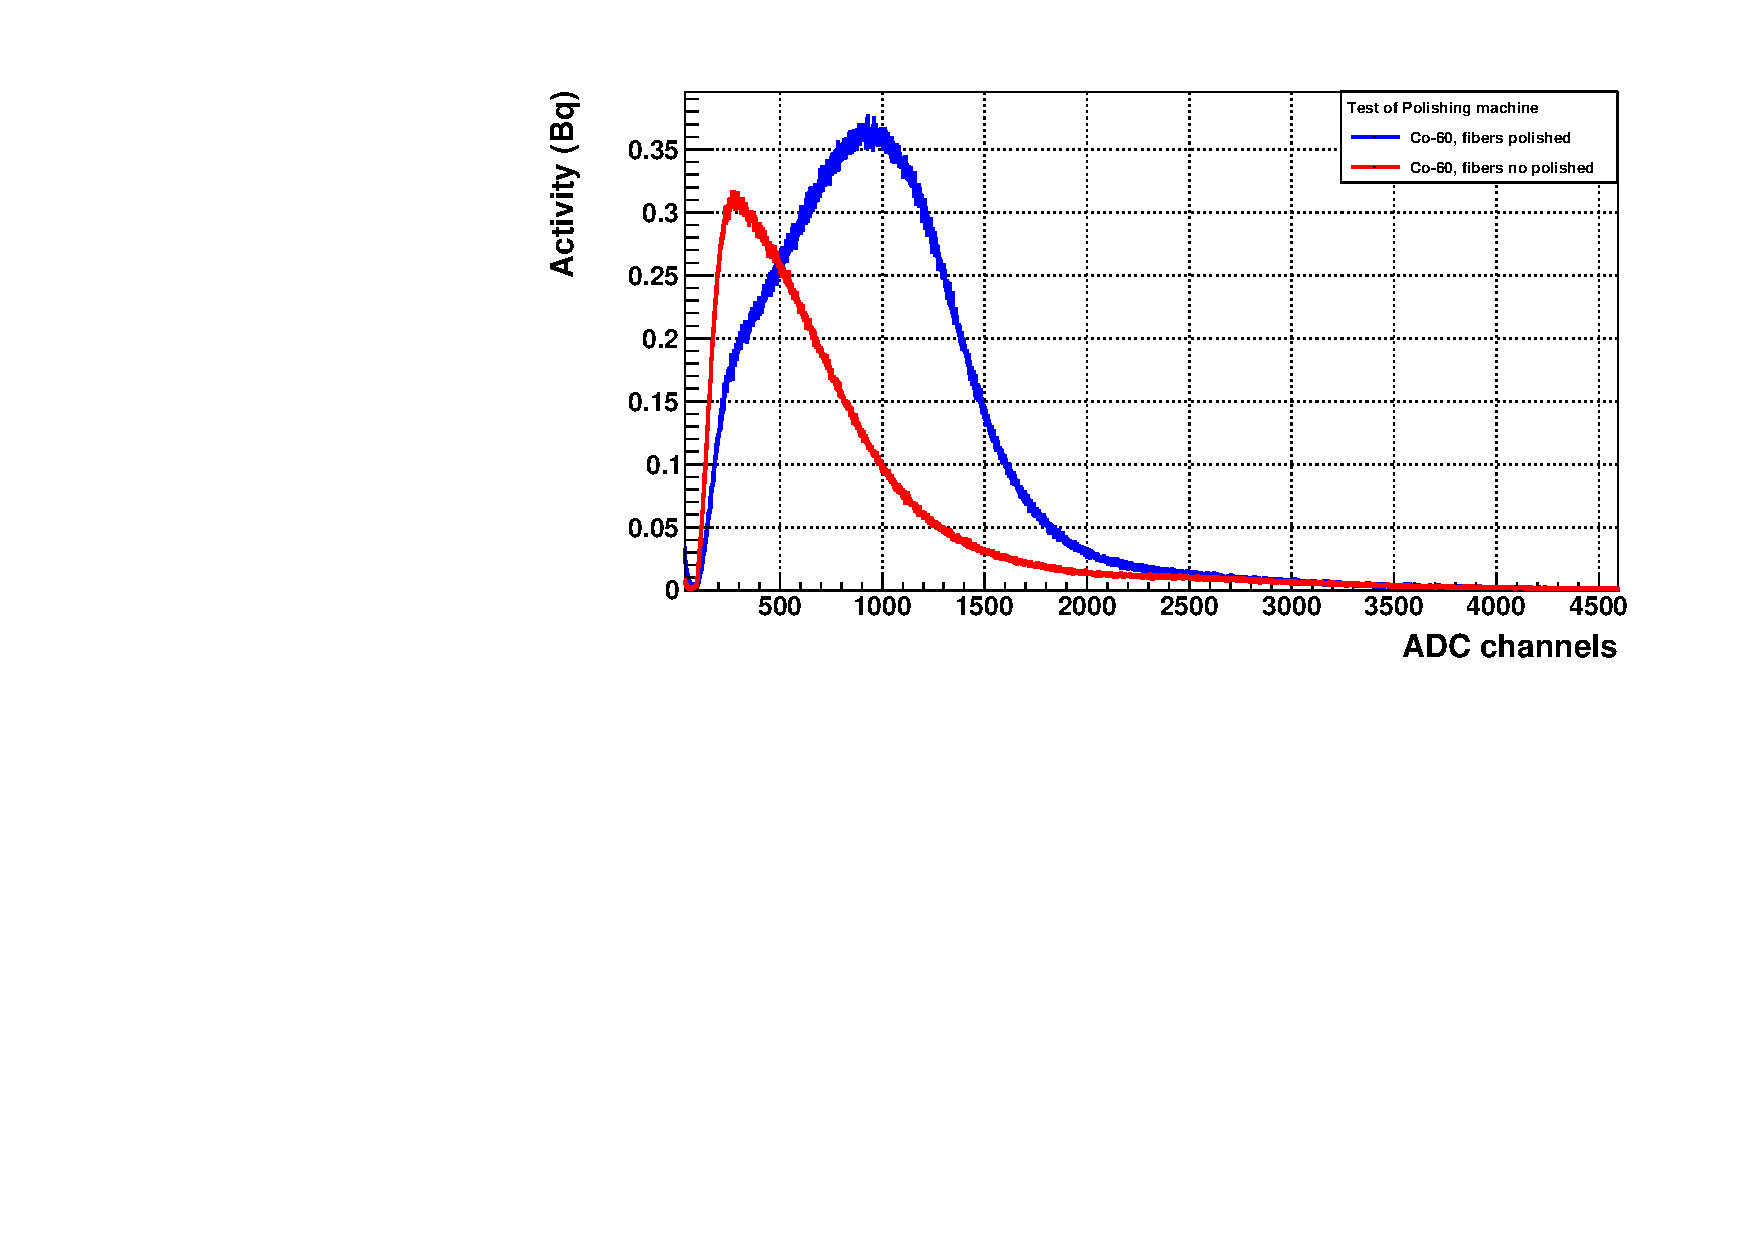
\includegraphics[width=\textwidth]{4ResearchAndDevelopments/41Fibers/Co_60_PolishingMachine_ZOOM.pdf}  
    \caption{\label{subfig:EnergySpectrumCo60PolishingTest}}
    \end{subfigure}
    \hfill
    \begin{subfigure}[b]{1\textwidth}
    \centering
    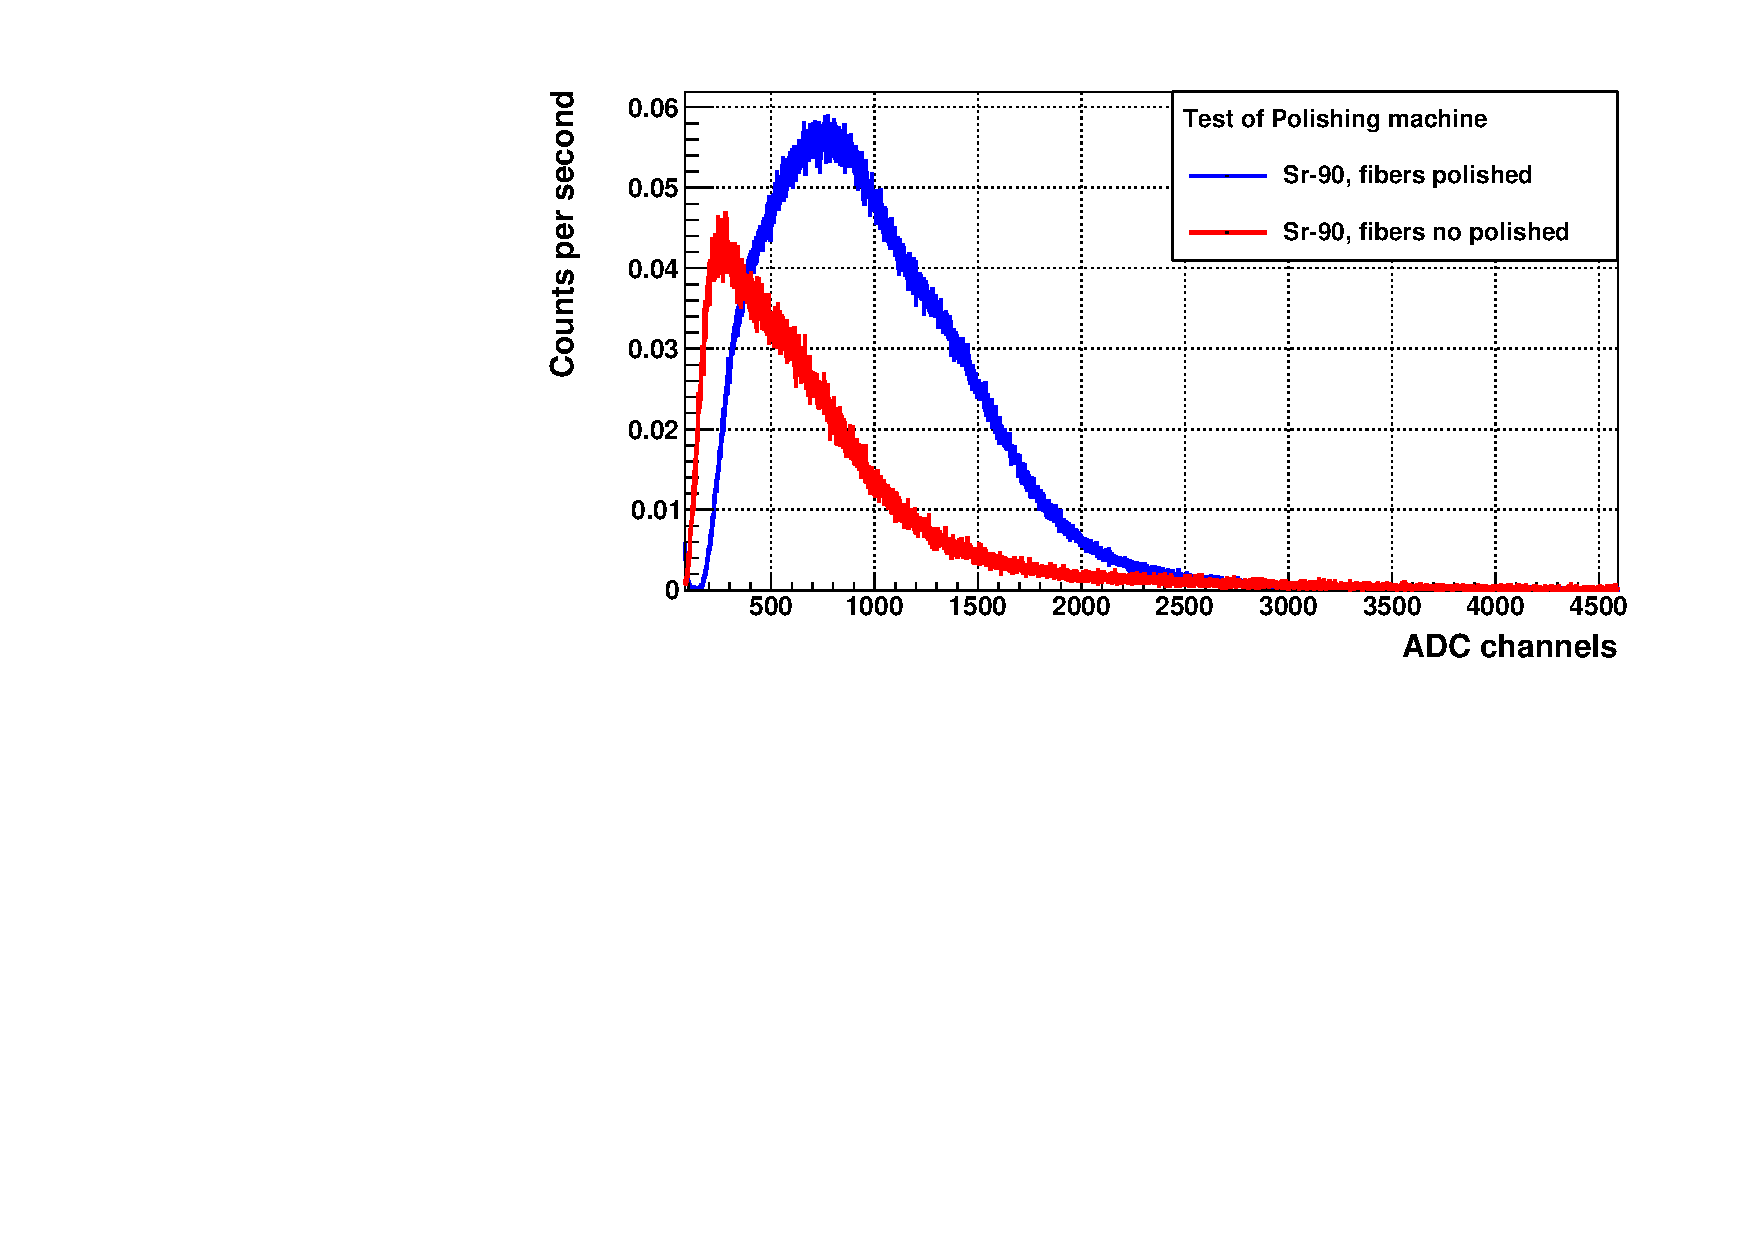
\includegraphics[width=\textwidth]{4ResearchAndDevelopments/41Fibers/Sr_90_PolishingMchine_ZOOM.pdf}  
    \caption{\label{subfig:EnergySpectrumSr90PolishingTest}}
    \end{subfigure}
 \caption{Energy spectra recorded with polished and unpolished fibers. a) $\ce{^{60}Co}$ source. b) $\ce{^{90}Sr}$ source.}
 \label{fig:ResultsOfPolishingMachineSources}
\end{figure}
It can be noticed that both energy spectra are shifted to the right after polishing, obtaining an improvement of a factor $1.7$ and $2$ with respect to the spectra before polishing for the $\ce{^{60}Co}$ and $\ce{^{90}Sr}$ sources, respectively. 

In summary, the photon collection efficiency of the fibers was significantly improved by polishing (mainly due to the improvement of the interface between fibers and PMTs). As the expected number of photons per tritium event is quite low (less than 20, as demonstrated by both simulations and measurements), it is crucial to achieve a high light collection.